\documentclass[1p]{elsarticle_modified}
%\bibliographystyle{elsarticle-num}

%\usepackage[colorlinks]{hyperref}
%\usepackage{abbrmath_seonhwa} %\Abb, \Ascr, \Acal ,\Abf, \Afrak
\usepackage{amsfonts}
\usepackage{amssymb}
\usepackage{amsmath}
\usepackage{amsthm}
\usepackage{scalefnt}
\usepackage{amsbsy}
\usepackage{kotex}
\usepackage{caption}
\usepackage{subfig}
\usepackage{color}
\usepackage{graphicx}
\usepackage{xcolor} %% white, black, red, green, blue, cyan, magenta, yellow
\usepackage{float}
\usepackage{setspace}
\usepackage{hyperref}

\usepackage{tikz}
\usetikzlibrary{arrows}

\usepackage{multirow}
\usepackage{array} % fixed length table
\usepackage{hhline}

%%%%%%%%%%%%%%%%%%%%%
\makeatletter
\renewcommand*\env@matrix[1][\arraystretch]{%
	\edef\arraystretch{#1}%
	\hskip -\arraycolsep
	\let\@ifnextchar\new@ifnextchar
	\array{*\c@MaxMatrixCols c}}
\makeatother %https://tex.stackexchange.com/questions/14071/how-can-i-increase-the-line-spacing-in-a-matrix
%%%%%%%%%%%%%%%

\usepackage[normalem]{ulem}

\newcommand{\msout}[1]{\ifmmode\text{\sout{\ensuremath{#1}}}\else\sout{#1}\fi}
%SOURCE: \msout is \stkout macro in https://tex.stackexchange.com/questions/20609/strikeout-in-math-mode

\newcommand{\cancel}[1]{
	\ifmmode
	{\color{red}\msout{#1}}
	\else
	{\color{red}\sout{#1}}
	\fi
}

\newcommand{\add}[1]{
	{\color{blue}\uwave{#1}}
}

\newcommand{\replace}[2]{
	\ifmmode
	{\color{red}\msout{#1}}{\color{blue}\uwave{#2}}
	\else
	{\color{red}\sout{#1}}{\color{blue}\uwave{#2}}
	\fi
}

\newcommand{\Sol}{\mathcal{S}} %segment
\newcommand{\D}{D} %diagram
\newcommand{\A}{\mathcal{A}} %arc


%%%%%%%%%%%%%%%%%%%%%%%%%%%%%5 test

\def\sl{\operatorname{\textup{SL}}(2,\Cbb)}
\def\psl{\operatorname{\textup{PSL}}(2,\Cbb)}
\def\quan{\mkern 1mu \triangleright \mkern 1mu}

\theoremstyle{definition}
\newtheorem{thm}{Theorem}[section]
\newtheorem{prop}[thm]{Proposition}
\newtheorem{lem}[thm]{Lemma}
\newtheorem{ques}[thm]{Question}
\newtheorem{cor}[thm]{Corollary}
\newtheorem{defn}[thm]{Definition}
\newtheorem{exam}[thm]{Example}
\newtheorem{rmk}[thm]{Remark}
\newtheorem{alg}[thm]{Algorithm}

\newcommand{\I}{\sqrt{-1}}
\begin{document}

%\begin{frontmatter}
%
%\title{Boundary parabolic representations of knots up to 8 crossings}
%
%%% Group authors per affiliation:
%\author{Yunhi Cho} 
%\address{Department of Mathematics, University of Seoul, Seoul, Korea}
%\ead{yhcho@uos.ac.kr}
%
%
%\author{Seonhwa Kim} %\fnref{s_kim}}
%\address{Center for Geometry and Physics, Institute for Basic Science, Pohang, 37673, Korea}
%\ead{ryeona17@ibs.re.kr}
%
%\author{Hyuk Kim}
%\address{Department of Mathematical Sciences, Seoul National University, Seoul 08826, Korea}
%\ead{hyukkim@snu.ac.kr}
%
%\author{Seokbeom Yoon}
%\address{Department of Mathematical Sciences, Seoul National University, Seoul, 08826,  Korea}
%\ead{sbyoon15@snu.ac.kr}
%
%\begin{abstract}
%We find all boundary parabolic representation of knots up to 8 crossings.
%
%\end{abstract}
%\begin{keyword}
%    \MSC[2010] 57M25 
%\end{keyword}
%
%\end{frontmatter}

%\linenumbers
%\tableofcontents
%
\newcommand\colored[1]{\textcolor{white}{\rule[-0.35ex]{0.8em}{1.4ex}}\kern-0.8em\color{red} #1}%
%\newcommand\colored[1]{\textcolor{white}{ #1}\kern-2.17ex	\textcolor{white}{ #1}\kern-1.81ex	\textcolor{white}{ #1}\kern-2.15ex\color{red}#1	}

{\Large $\underline{12n_{0626}~(K12n_{0626})}$}

\setlength{\tabcolsep}{10pt}
\renewcommand{\arraystretch}{1.6}
\vspace{1cm}\begin{tabular}{m{100pt}>{\centering\arraybackslash}m{274pt}}
\multirow{5}{120pt}{
	\centering
	\includegraphics[width=112pt]{../../../GIT/diagram.site/Diagrams/png/2715_12n_0626.png}\\
\ \ \ A knot diagram\footnotemark}&
\allowdisplaybreaks
\textbf{Linearized knot diagam} \\
\cline{2-2}
 &
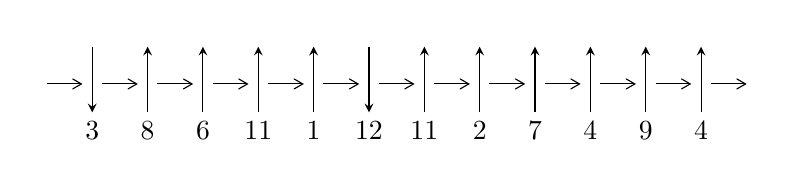
\begin{tikzpicture}[x=20pt, y=17pt]
	% nodes
	\node (C0) at (0, 0) {};
	\node (C1) at (1, 0) {};
	\node (C1U) at (1, +1) {};
	\node (C1D) at (1, -1) {3};

	\node (C2) at (2, 0) {};
	\node (C2U) at (2, +1) {};
	\node (C2D) at (2, -1) {8};

	\node (C3) at (3, 0) {};
	\node (C3U) at (3, +1) {};
	\node (C3D) at (3, -1) {6};

	\node (C4) at (4, 0) {};
	\node (C4U) at (4, +1) {};
	\node (C4D) at (4, -1) {11};

	\node (C5) at (5, 0) {};
	\node (C5U) at (5, +1) {};
	\node (C5D) at (5, -1) {1};

	\node (C6) at (6, 0) {};
	\node (C6U) at (6, +1) {};
	\node (C6D) at (6, -1) {12};

	\node (C7) at (7, 0) {};
	\node (C7U) at (7, +1) {};
	\node (C7D) at (7, -1) {11};

	\node (C8) at (8, 0) {};
	\node (C8U) at (8, +1) {};
	\node (C8D) at (8, -1) {2};

	\node (C9) at (9, 0) {};
	\node (C9U) at (9, +1) {};
	\node (C9D) at (9, -1) {7};

	\node (C10) at (10, 0) {};
	\node (C10U) at (10, +1) {};
	\node (C10D) at (10, -1) {4};

	\node (C11) at (11, 0) {};
	\node (C11U) at (11, +1) {};
	\node (C11D) at (11, -1) {9};

	\node (C12) at (12, 0) {};
	\node (C12U) at (12, +1) {};
	\node (C12D) at (12, -1) {4};
	\node (C13) at (13, 0) {};

	% arrows
	\draw[->,>={angle 60}]
	(C0) edge (C1) (C1) edge (C2) (C2) edge (C3) (C3) edge (C4) (C4) edge (C5) (C5) edge (C6) (C6) edge (C7) (C7) edge (C8) (C8) edge (C9) (C9) edge (C10) (C10) edge (C11) (C11) edge (C12) (C12) edge (C13) ;	\draw[->,>=stealth]
	(C1U) edge (C1D) (C2D) edge (C2U) (C3D) edge (C3U) (C4D) edge (C4U) (C5D) edge (C5U) (C6U) edge (C6D) (C7D) edge (C7U) (C8D) edge (C8U) (C9D) edge (C9U) (C10D) edge (C10U) (C11D) edge (C11U) (C12D) edge (C12U) ;
	\end{tikzpicture} \\
\hhline{~~} \\& 
\textbf{Solving Sequence} \\ \cline{2-2} 
 &
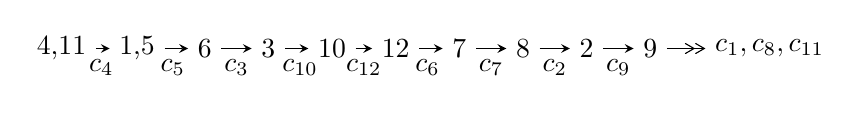
\begin{tikzpicture}[x=23pt, y=7pt]
	% node
	\node (A0) at (-1/8, 0) {4,11};
	\node (A1) at (17/16, 0) {1,5};
	\node (A2) at (17/8, 0) {6};
	\node (A3) at (25/8, 0) {3};
	\node (A4) at (33/8, 0) {10};
	\node (A5) at (41/8, 0) {12};
	\node (A6) at (49/8, 0) {7};
	\node (A7) at (57/8, 0) {8};
	\node (A8) at (65/8, 0) {2};
	\node (A9) at (73/8, 0) {9};
	\node (C1) at (1/2, -1) {$c_{4}$};
	\node (C2) at (13/8, -1) {$c_{5}$};
	\node (C3) at (21/8, -1) {$c_{3}$};
	\node (C4) at (29/8, -1) {$c_{10}$};
	\node (C5) at (37/8, -1) {$c_{12}$};
	\node (C6) at (45/8, -1) {$c_{6}$};
	\node (C7) at (53/8, -1) {$c_{7}$};
	\node (C8) at (61/8, -1) {$c_{2}$};
	\node (C9) at (69/8, -1) {$c_{9}$};
	\node (A10) at (11, 0) {$c_{1},c_{8},c_{11}$};

	% edge
	\draw[->,>=stealth]	
	(A0) edge (A1) (A1) edge (A2) (A2) edge (A3) (A3) edge (A4) (A4) edge (A5) (A5) edge (A6) (A6) edge (A7) (A7) edge (A8) (A8) edge (A9) ;
	\draw[->>,>={angle 60}]	
	(A9) edge (A10);
\end{tikzpicture} \\ 

\end{tabular} \\

\footnotetext{
The image of knot diagram is generated by the software ``\textbf{Draw programme}" developed by Andrew Bartholomew(\url{http://www.layer8.co.uk/maths/draw/index.htm\#Running-draw}), where we modified some parts for our purpose(\url{https://github.com/CATsTAILs/LinksPainter}).
}\phantom \\ \newline 
\centering \textbf{Ideals for irreducible components\footnotemark of $X_{\text{par}}$} 
 
\begin{align*}
I^u_{1}&=\langle 
6.45261\times10^{107} u^{44}-2.43067\times10^{108} u^{43}+\cdots+5.67762\times10^{109} b+1.45136\times10^{110},\\
\phantom{I^u_{1}}&\phantom{= \langle  }-1.02261\times10^{111} u^{44}+3.49755\times10^{111} u^{43}+\cdots+3.12269\times10^{112} a-1.77035\times10^{113},\\
\phantom{I^u_{1}}&\phantom{= \langle  }u^{45}-3 u^{44}+\cdots-216 u-50\rangle \\
I^u_{2}&=\langle 
-1.57405\times10^{49} a u^{34}-7.29045\times10^{49} u^{34}+\cdots-1.01763\times10^{50} a-5.06550\times10^{50},\\
\phantom{I^u_{2}}&\phantom{= \langle  }4.89851\times10^{51} a u^{34}-1.12145\times10^{52} u^{34}+\cdots+3.20904\times10^{52} a-7.96667\times10^{52},\;u^{35}+u^{34}+\cdots+9 u-1\rangle \\
I^u_{3}&=\langle 
24290268766301 u^{37}-28827427845386 u^{36}+\cdots+64246238253402 b+686511198649974,\\
\phantom{I^u_{3}}&\phantom{= \langle  }-193561107143803 u^{37}+110734887539683 u^{36}+\cdots+64246238253402 a-901423536620652,\\
\phantom{I^u_{3}}&\phantom{= \langle  }u^{38}+5 u^{36}+\cdots-71 u^2+6\rangle \\
\\
I^v_{1}&=\langle 
a,\;b-1,\;v+1\rangle \\
\end{align*}
\raggedright * 4 irreducible components of $\dim_{\mathbb{C}}=0$, with total 154 representations.\\
\footnotetext{All coefficients of polynomials are rational numbers. But the coefficients are sometimes approximated in decimal forms when there is not enough margin.}
\newpage
\renewcommand{\arraystretch}{1}
\centering \section*{I. $I^u_{1}= \langle 6.45\times10^{107} u^{44}-2.43\times10^{108} u^{43}+\cdots+5.68\times10^{109} b+1.45\times10^{110},\;-1.02\times10^{111} u^{44}+3.50\times10^{111} u^{43}+\cdots+3.12\times10^{112} a-1.77\times10^{113},\;u^{45}-3 u^{44}+\cdots-216 u-50 \rangle$}
\flushleft \textbf{(i) Arc colorings}\\
\begin{tabular}{m{7pt} m{180pt} m{7pt} m{180pt} }
\flushright $a_{4}=$&$\begin{pmatrix}1\\0\end{pmatrix}$ \\
\flushright $a_{11}=$&$\begin{pmatrix}0\\u\end{pmatrix}$ \\
\flushright $a_{1}=$&$\begin{pmatrix}0.0327477 u^{44}-0.112004 u^{43}+\cdots+14.6356 u+5.66930\\-0.0113650 u^{44}+0.0428114 u^{43}+\cdots-7.23755 u-2.55629\end{pmatrix}$ \\
\flushright $a_{5}=$&$\begin{pmatrix}1\\- u^2\end{pmatrix}$ \\
\flushright $a_{6}=$&$\begin{pmatrix}0.000138274 u^{44}-0.0215805 u^{43}+\cdots+48.5815 u+14.2524\\-0.00976057 u^{44}+0.0369257 u^{43}+\cdots-11.2636 u-3.57324\end{pmatrix}$ \\
\flushright $a_{3}=$&$\begin{pmatrix}0.0549640 u^{44}-0.133609 u^{43}+\cdots-78.7955 u-12.0431\\-0.0224776 u^{44}+0.0618353 u^{43}+\cdots+17.7539 u+2.20564\end{pmatrix}$ \\
\flushright $a_{10}=$&$\begin{pmatrix}- u\\u\end{pmatrix}$ \\
\flushright $a_{12}=$&$\begin{pmatrix}0.0441127 u^{44}-0.154816 u^{43}+\cdots+21.8732 u+8.22559\\-0.0113650 u^{44}+0.0428114 u^{43}+\cdots-7.23755 u-2.55629\end{pmatrix}$ \\
\flushright $a_{7}=$&$\begin{pmatrix}-0.0648870 u^{44}+0.178186 u^{43}+\cdots+48.2969 u+5.44301\\0.0137612 u^{44}-0.0361735 u^{43}+\cdots-12.7428 u-1.63739\end{pmatrix}$ \\
\flushright $a_{8}=$&$\begin{pmatrix}-0.0648870 u^{44}+0.178186 u^{43}+\cdots+48.2969 u+5.44301\\0.00125770 u^{44}+0.00211282 u^{43}+\cdots-5.93985 u-0.813634\end{pmatrix}$ \\
\flushright $a_{2}=$&$\begin{pmatrix}-0.0253004 u^{44}+0.110341 u^{43}+\cdots-46.4915 u-11.6489\\-0.00636661 u^{44}+0.0145163 u^{43}+\cdots+13.8908 u+2.19911\end{pmatrix}$ \\
\flushright $a_{9}=$&$\begin{pmatrix}-0.0714648 u^{44}+0.204634 u^{43}+\cdots+46.2269 u+4.17282\\0.0149532 u^{44}-0.0451343 u^{43}+\cdots-8.51402 u+0.0701677\end{pmatrix}$\\&\end{tabular}
\flushleft \textbf{(ii) Obstruction class $= -1$}\\~\\
\flushleft \textbf{(iii) Cusp Shapes $= 0.0618399 u^{44}-0.112199 u^{43}+\cdots-99.5480 u-9.36086$}\\~\\
\newpage\renewcommand{\arraystretch}{1}
\flushleft \textbf{(iv) u-Polynomials at the component}\newline \\
\begin{tabular}{m{50pt}|m{274pt}}
Crossings & \hspace{64pt}u-Polynomials at each crossing \\
\hline $$\begin{aligned}c_{1}\end{aligned}$$&$\begin{aligned}
&u^{45}+19 u^{44}+\cdots+296 u-100
\end{aligned}$\\
\hline $$\begin{aligned}c_{2},c_{8}\end{aligned}$$&$\begin{aligned}
&u^{45}+3 u^{44}+\cdots-44 u-10
\end{aligned}$\\
\hline $$\begin{aligned}c_{3},c_{11}\end{aligned}$$&$\begin{aligned}
&u^{45}+u^{44}+\cdots+5 u-1
\end{aligned}$\\
\hline $$\begin{aligned}c_{4},c_{10}\end{aligned}$$&$\begin{aligned}
&u^{45}-3 u^{44}+\cdots-216 u-50
\end{aligned}$\\
\hline $$\begin{aligned}c_{5},c_{7}\end{aligned}$$&$\begin{aligned}
&u^{45}- u^{44}+\cdots+11 u-143
\end{aligned}$\\
\hline $$\begin{aligned}c_{6}\end{aligned}$$&$\begin{aligned}
&u^{45}-3 u^{44}+\cdots+8824 u-1928
\end{aligned}$\\
\hline $$\begin{aligned}c_{9},c_{12}\end{aligned}$$&$\begin{aligned}
&u^{45}+3 u^{44}+\cdots+33 u-16
\end{aligned}$\\
\hline
\end{tabular}\\~\\
\newpage\renewcommand{\arraystretch}{1}
\flushleft \textbf{(v) Riley Polynomials at the component}\newline \\
\begin{tabular}{m{50pt}|m{274pt}}
Crossings & \hspace{64pt}Riley Polynomials at each crossing \\
\hline $$\begin{aligned}c_{1}\end{aligned}$$&$\begin{aligned}
&y^{45}+15 y^{44}+\cdots+417216 y-10000
\end{aligned}$\\
\hline $$\begin{aligned}c_{2},c_{8}\end{aligned}$$&$\begin{aligned}
&y^{45}+19 y^{44}+\cdots+296 y-100
\end{aligned}$\\
\hline $$\begin{aligned}c_{3},c_{11}\end{aligned}$$&$\begin{aligned}
&y^{45}-7 y^{44}+\cdots+25 y-1
\end{aligned}$\\
\hline $$\begin{aligned}c_{4},c_{10}\end{aligned}$$&$\begin{aligned}
&y^{45}+29 y^{44}+\cdots-66944 y-2500
\end{aligned}$\\
\hline $$\begin{aligned}c_{5},c_{7}\end{aligned}$$&$\begin{aligned}
&y^{45}+27 y^{44}+\cdots-283019 y-20449
\end{aligned}$\\
\hline $$\begin{aligned}c_{6}\end{aligned}$$&$\begin{aligned}
&y^{45}-5 y^{44}+\cdots+32639808 y-3717184
\end{aligned}$\\
\hline $$\begin{aligned}c_{9},c_{12}\end{aligned}$$&$\begin{aligned}
&y^{45}+35 y^{44}+\cdots-6847 y-256
\end{aligned}$\\
\hline
\end{tabular}\\~\\
\newpage\flushleft \textbf{(vi) Complex Volumes and Cusp Shapes}
$$\begin{array}{c|c|c}  
\text{Solutions to }I^u_{1}& \I (\text{vol} + \sqrt{-1}CS) & \text{Cusp shape}\\
 \hline 
\begin{aligned}
u &= \phantom{-}0.982052 + 0.344463 I \\
a &= \phantom{-}0.897344 + 0.387946 I \\
b &= -0.088808 - 0.284640 I\end{aligned}
 & \phantom{-}3.90111 + 0.24103 I & \phantom{-}11.14977 - 0.22983 I \\ \hline\begin{aligned}
u &= \phantom{-}0.982052 - 0.344463 I \\
a &= \phantom{-}0.897344 - 0.387946 I \\
b &= -0.088808 + 0.284640 I\end{aligned}
 & \phantom{-}3.90111 - 0.24103 I & \phantom{-}11.14977 + 0.22983 I \\ \hline\begin{aligned}
u &= -0.972469 + 0.418664 I \\
a &= -0.875723 + 0.572022 I \\
b &= \phantom{-}0.215420 - 0.332153 I\end{aligned}
 & \phantom{-}3.69660 - 5.52791 I & \phantom{-}11.56773 + 6.24960 I \\ \hline\begin{aligned}
u &= -0.972469 - 0.418664 I \\
a &= -0.875723 - 0.572022 I \\
b &= \phantom{-}0.215420 + 0.332153 I\end{aligned}
 & \phantom{-}3.69660 + 5.52791 I & \phantom{-}11.56773 - 6.24960 I \\ \hline\begin{aligned}
u &= -0.268181 + 1.172890 I \\
a &= -1.099600 - 0.836869 I \\
b &= -1.32797 - 1.27587 I\end{aligned}
 & -4.61487 - 1.65819 I & -5.41137 + 0.80754 I \\ \hline\begin{aligned}
u &= -0.268181 - 1.172890 I \\
a &= -1.099600 + 0.836869 I \\
b &= -1.32797 + 1.27587 I\end{aligned}
 & -4.61487 + 1.65819 I & -5.41137 - 0.80754 I \\ \hline\begin{aligned}
u &= -0.133716 + 1.210450 I \\
a &= \phantom{-}0.46886 - 1.72677 I \\
b &= \phantom{-}1.06503 - 1.77331 I\end{aligned}
 & -1.11353 - 5.69606 I & \phantom{-}6.4348 + 13.2641 I \\ \hline\begin{aligned}
u &= -0.133716 - 1.210450 I \\
a &= \phantom{-}0.46886 + 1.72677 I \\
b &= \phantom{-}1.06503 + 1.77331 I\end{aligned}
 & -1.11353 + 5.69606 I & \phantom{-}6.4348 - 13.2641 I \\ \hline\begin{aligned}
u &= \phantom{-}0.133959 + 1.289230 I \\
a &= -0.30874 + 1.56623 I \\
b &= -0.35217 + 1.59122 I\end{aligned}
 & -3.03297 + 3.57228 I & \phantom{-}2.57196 - 5.14807 I \\ \hline\begin{aligned}
u &= \phantom{-}0.133959 - 1.289230 I \\
a &= -0.30874 - 1.56623 I \\
b &= -0.35217 - 1.59122 I\end{aligned}
 & -3.03297 - 3.57228 I & \phantom{-}2.57196 + 5.14807 I\\
 \hline 
 \end{array}$$\newpage$$\begin{array}{c|c|c}  
\text{Solutions to }I^u_{1}& \I (\text{vol} + \sqrt{-1}CS) & \text{Cusp shape}\\
 \hline 
\begin{aligned}
u &= -0.381503 + 1.269590 I \\
a &= \phantom{-}0.440182 + 0.942074 I \\
b &= -0.322936 + 1.028520 I\end{aligned}
 & -3.88171 + 0.13510 I & \phantom{-}6.67770 - 1.97779 I \\ \hline\begin{aligned}
u &= -0.381503 - 1.269590 I \\
a &= \phantom{-}0.440182 - 0.942074 I \\
b &= -0.322936 - 1.028520 I\end{aligned}
 & -3.88171 - 0.13510 I & \phantom{-}6.67770 + 1.97779 I \\ \hline\begin{aligned}
u &= \phantom{-}0.018489 + 1.337230 I \\
a &= \phantom{-}0.584739 + 1.185070 I \\
b &= -0.133197 + 0.864237 I\end{aligned}
 & -2.93966 + 2.29015 I & \phantom{-}3.98465 - 3.47136 I \\ \hline\begin{aligned}
u &= \phantom{-}0.018489 - 1.337230 I \\
a &= \phantom{-}0.584739 - 1.185070 I \\
b &= -0.133197 - 0.864237 I\end{aligned}
 & -2.93966 - 2.29015 I & \phantom{-}3.98465 + 3.47136 I \\ \hline\begin{aligned}
u &= -0.537745 + 0.270263 I \\
a &= \phantom{-}1.193340 - 0.691780 I \\
b &= \phantom{-}0.823079 + 0.760072 I\end{aligned}
 & \phantom{-}1.78194 + 3.46593 I & \phantom{-}14.6287 - 5.6907 I \\ \hline\begin{aligned}
u &= -0.537745 - 0.270263 I \\
a &= \phantom{-}1.193340 + 0.691780 I \\
b &= \phantom{-}0.823079 - 0.760072 I\end{aligned}
 & \phantom{-}1.78194 - 3.46593 I & \phantom{-}14.6287 + 5.6907 I \\ \hline\begin{aligned}
u &= -0.06352 + 1.41822 I \\
a &= -0.577294 + 1.275210 I \\
b &= \phantom{-}0.084859 + 0.840729 I\end{aligned}
 & -4.25393 - 7.67261 I & \phantom{-0.000000 -}0. + 9.08596 I \\ \hline\begin{aligned}
u &= -0.06352 - 1.41822 I \\
a &= -0.577294 - 1.275210 I \\
b &= \phantom{-}0.084859 - 0.840729 I\end{aligned}
 & -4.25393 + 7.67261 I & \phantom{-0.000000 } 0. - 9.08596 I \\ \hline\begin{aligned}
u &= -0.481194 + 0.313751 I \\
a &= -0.59895 + 1.71117 I \\
b &= \phantom{-}0.662716 - 0.478922 I\end{aligned}
 & \phantom{-}1.48372 - 3.19466 I & \phantom{-}14.2637 + 3.1183 I \\ \hline\begin{aligned}
u &= -0.481194 - 0.313751 I \\
a &= -0.59895 - 1.71117 I \\
b &= \phantom{-}0.662716 + 0.478922 I\end{aligned}
 & \phantom{-}1.48372 + 3.19466 I & \phantom{-}14.2637 - 3.1183 I\\
 \hline 
 \end{array}$$\newpage$$\begin{array}{c|c|c}  
\text{Solutions to }I^u_{1}& \I (\text{vol} + \sqrt{-1}CS) & \text{Cusp shape}\\
 \hline 
\begin{aligned}
u &= \phantom{-}1.45205 + 0.30573 I \\
a &= \phantom{-}0.189061 + 0.075403 I \\
b &= -0.202622 - 1.155420 I\end{aligned}
 & -1.85503 + 3.23232 I & \phantom{-0.000000 } 0 \\ \hline\begin{aligned}
u &= \phantom{-}1.45205 - 0.30573 I \\
a &= \phantom{-}0.189061 - 0.075403 I \\
b &= -0.202622 + 1.155420 I\end{aligned}
 & -1.85503 - 3.23232 I & \phantom{-0.000000 } 0 \\ \hline\begin{aligned}
u &= \phantom{-}0.11068 + 1.49218 I \\
a &= -0.362471 + 1.218380 I \\
b &= \phantom{-}0.021640 + 1.003810 I\end{aligned}
 & -8.41188 - 1.42060 I & \phantom{-0.000000 } 0 \\ \hline\begin{aligned}
u &= \phantom{-}0.11068 - 1.49218 I \\
a &= -0.362471 - 1.218380 I \\
b &= \phantom{-}0.021640 - 1.003810 I\end{aligned}
 & -8.41188 + 1.42060 I & \phantom{-0.000000 } 0 \\ \hline\begin{aligned}
u &= -0.352040 + 0.357974 I \\
a &= \phantom{-}0.018861 + 1.267180 I \\
b &= -0.675952 + 0.468271 I\end{aligned}
 & -2.55936 - 1.04400 I & \phantom{-}3.67071 + 4.11672 I \\ \hline\begin{aligned}
u &= -0.352040 - 0.357974 I \\
a &= \phantom{-}0.018861 - 1.267180 I \\
b &= -0.675952 - 0.468271 I\end{aligned}
 & -2.55936 + 1.04400 I & \phantom{-}3.67071 - 4.11672 I \\ \hline\begin{aligned}
u &= -1.46794 + 0.33452 I \\
a &= \phantom{-}0.1160420 + 0.0084688 I \\
b &= \phantom{-}0.584119 + 1.190960 I\end{aligned}
 & \phantom{-}2.62425 + 5.00892 I & \phantom{-0.000000 } 0 \\ \hline\begin{aligned}
u &= -1.46794 - 0.33452 I \\
a &= \phantom{-}0.1160420 - 0.0084688 I \\
b &= \phantom{-}0.584119 - 1.190960 I\end{aligned}
 & \phantom{-}2.62425 - 5.00892 I & \phantom{-0.000000 } 0 \\ \hline\begin{aligned}
u &= \phantom{-}0.457354\phantom{ +0.000000I} \\
a &= \phantom{-}0.515813\phantom{ +0.000000I} \\
b &= \phantom{-}0.287710\phantom{ +0.000000I}\end{aligned}
 & \phantom{-}0.695378\phantom{ +0.000000I} & \phantom{-}13.8950\phantom{ +0.000000I} \\ \hline\begin{aligned}
u &= \phantom{-}0.71712 + 1.42041 I \\
a &= -0.377061 + 0.827181 I \\
b &= \phantom{-}0.458019 + 1.197090 I\end{aligned}
 & -5.71574 + 4.33440 I & \phantom{-0.000000 } 0\\
 \hline 
 \end{array}$$\newpage$$\begin{array}{c|c|c}  
\text{Solutions to }I^u_{1}& \I (\text{vol} + \sqrt{-1}CS) & \text{Cusp shape}\\
 \hline 
\begin{aligned}
u &= \phantom{-}0.71712 - 1.42041 I \\
a &= -0.377061 - 0.827181 I \\
b &= \phantom{-}0.458019 - 1.197090 I\end{aligned}
 & -5.71574 - 4.33440 I & \phantom{-0.000000 } 0 \\ \hline\begin{aligned}
u &= \phantom{-}0.045115 + 0.375785 I \\
a &= \phantom{-}0.502574 - 0.452745 I \\
b &= -0.076285 + 0.710609 I\end{aligned}
 & \phantom{-}1.59089 + 2.72032 I & \phantom{-}6.64779 - 2.49427 I \\ \hline\begin{aligned}
u &= \phantom{-}0.045115 - 0.375785 I \\
a &= \phantom{-}0.502574 + 0.452745 I \\
b &= -0.076285 - 0.710609 I\end{aligned}
 & \phantom{-}1.59089 - 2.72032 I & \phantom{-}6.64779 + 2.49427 I \\ \hline\begin{aligned}
u &= \phantom{-}0.37049 + 1.59283 I \\
a &= -0.049575 - 1.215240 I \\
b &= -1.06311 - 1.54495 I\end{aligned}
 & -8.64456 + 9.60665 I & \phantom{-0.000000 } 0 \\ \hline\begin{aligned}
u &= \phantom{-}0.37049 - 1.59283 I \\
a &= -0.049575 + 1.215240 I \\
b &= -1.06311 + 1.54495 I\end{aligned}
 & -8.64456 - 9.60665 I & \phantom{-0.000000 } 0 \\ \hline\begin{aligned}
u &= -0.68867 + 1.49281 I \\
a &= -0.230013 - 1.255740 I \\
b &= \phantom{-}1.03402 - 1.44601 I\end{aligned}
 & -1.39112 - 12.65970 I & \phantom{-0.000000 } 0 \\ \hline\begin{aligned}
u &= -0.68867 - 1.49281 I \\
a &= -0.230013 + 1.255740 I \\
b &= \phantom{-}1.03402 + 1.44601 I\end{aligned}
 & -1.39112 + 12.65970 I & \phantom{-0.000000 } 0 \\ \hline\begin{aligned}
u &= \phantom{-}0.008729 + 0.329890 I \\
a &= \phantom{-}2.99643 + 1.73672 I \\
b &= -0.844063 - 0.436623 I\end{aligned}
 & \phantom{-}0.04511 + 7.55751 I & \phantom{-}10.37988 - 8.84114 I \\ \hline\begin{aligned}
u &= \phantom{-}0.008729 - 0.329890 I \\
a &= \phantom{-}2.99643 - 1.73672 I \\
b &= -0.844063 + 0.436623 I\end{aligned}
 & \phantom{-}0.04511 - 7.55751 I & \phantom{-}10.37988 + 8.84114 I \\ \hline\begin{aligned}
u &= \phantom{-}0.78407 + 1.59419 I \\
a &= \phantom{-}0.265720 - 1.158860 I \\
b &= -1.07883 - 1.42333 I\end{aligned}
 & -3.5107 + 18.8570 I & \phantom{-0.000000 } 0\\
 \hline 
 \end{array}$$\newpage$$\begin{array}{c|c|c}  
\text{Solutions to }I^u_{1}& \I (\text{vol} + \sqrt{-1}CS) & \text{Cusp shape}\\
 \hline 
\begin{aligned}
u &= \phantom{-}0.78407 - 1.59419 I \\
a &= \phantom{-}0.265720 + 1.158860 I \\
b &= -1.07883 + 1.42333 I\end{aligned}
 & -3.5107 - 18.8570 I & \phantom{-0.000000 } 0 \\ \hline\begin{aligned}
u &= \phantom{-}1.76555 + 0.27957 I \\
a &= -0.0198463 + 0.0768389 I \\
b &= -0.54488 + 1.32858 I\end{aligned}
 & \phantom{-}0.87619 - 10.06840 I & \phantom{-0.000000 } 0 \\ \hline\begin{aligned}
u &= \phantom{-}1.76555 - 0.27957 I \\
a &= -0.0198463 - 0.0768389 I \\
b &= -0.54488 - 1.32858 I\end{aligned}
 & \phantom{-}0.87619 + 10.06840 I & \phantom{-0.000000 } 0 \\ \hline\begin{aligned}
u &= \phantom{-}0.23000 + 2.00315 I \\
a &= -0.091790 + 0.847105 I \\
b &= \phantom{-}0.11807 + 1.45362 I\end{aligned}
 & -7.19068 - 1.47568 I & \phantom{-0.000000 } 0 \\ \hline\begin{aligned}
u &= \phantom{-}0.23000 - 2.00315 I \\
a &= -0.091790 - 0.847105 I \\
b &= \phantom{-}0.11807 - 1.45362 I\end{aligned}
 & -7.19068 + 1.47568 I & \phantom{-0.000000 } 0\\
 \hline 
 \end{array}$$\newpage\newpage\renewcommand{\arraystretch}{1}
\centering \section*{II. $I^u_{2}= \langle -1.57\times10^{49} a u^{34}-7.29\times10^{49} u^{34}+\cdots-1.02\times10^{50} a-5.07\times10^{50},\;4.90\times10^{51} a u^{34}-1.12\times10^{52} u^{34}+\cdots+3.21\times10^{52} a-7.97\times10^{52},\;u^{35}+u^{34}+\cdots+9 u-1 \rangle$}
\flushleft \textbf{(i) Arc colorings}\\
\begin{tabular}{m{7pt} m{180pt} m{7pt} m{180pt} }
\flushright $a_{4}=$&$\begin{pmatrix}1\\0\end{pmatrix}$ \\
\flushright $a_{11}=$&$\begin{pmatrix}0\\u\end{pmatrix}$ \\
\flushright $a_{1}=$&$\begin{pmatrix}a\\0.0958186 a u^{34}+0.443798 u^{34}+\cdots+0.619469 a+3.08357\end{pmatrix}$ \\
\flushright $a_{5}=$&$\begin{pmatrix}1\\- u^2\end{pmatrix}$ \\
\flushright $a_{6}=$&$\begin{pmatrix}1.41657 a u^{34}-6.79284 u^{34}+\cdots+9.76303 a-47.0037\\0.132146 a u^{34}+1.39494 u^{34}+\cdots+0.980193 a+8.18591\end{pmatrix}$ \\
\flushright $a_{3}=$&$\begin{pmatrix}1.32752 a u^{34}+6.79284 u^{34}+\cdots+9.36987 a+47.0037\\0.0201917 a u^{34}-4.25432 u^{34}+\cdots+0.0958186 a-28.9986\end{pmatrix}$ \\
\flushright $a_{10}=$&$\begin{pmatrix}- u\\u\end{pmatrix}$ \\
\flushright $a_{12}=$&$\begin{pmatrix}-0.0958186 a u^{34}-0.443798 u^{34}+\cdots+0.380531 a-3.08357\\0.0958186 a u^{34}+0.443798 u^{34}+\cdots+0.619469 a+3.08357\end{pmatrix}$ \\
\flushright $a_{7}=$&$\begin{pmatrix}-0.619469 a u^{34}-9.76303 u^{34}+\cdots-4.12036 a-68.6369\\4.36514 u^{34}+4.96123 u^{33}+\cdots-73.0252 u+29.8191\end{pmatrix}$ \\
\flushright $a_{8}=$&$\begin{pmatrix}-0.619469 a u^{34}-9.76303 u^{34}+\cdots-4.12036 a-68.6369\\0.0201917 a u^{34}+4.57371 u^{34}+\cdots+0.0958186 a+31.2357\end{pmatrix}$ \\
\flushright $a_{2}=$&$\begin{pmatrix}1.55451 a u^{34}-2.98159 u^{34}+\cdots+10.6192 a-22.8488\\-0.180352 a u^{34}+0.0676458 u^{34}+\cdots-1.24871 a+0.423180\end{pmatrix}$ \\
\flushright $a_{9}=$&$\begin{pmatrix}-0.980193 a u^{34}+u^{34}+\cdots-7.39826 a+9\\0.110817 a u^{34}-0.212265 u^{34}+\cdots+0.820472 a-1.03387\end{pmatrix}$\\&\end{tabular}
\flushleft \textbf{(ii) Obstruction class $= -1$}\\~\\
\flushleft \textbf{(iii) Cusp Shapes $= 3.08049 u^{34}+3.61372 u^{33}+\cdots-30.9682 u+20.7546$}\\~\\
\newpage\renewcommand{\arraystretch}{1}
\flushleft \textbf{(iv) u-Polynomials at the component}\newline \\
\begin{tabular}{m{50pt}|m{274pt}}
Crossings & \hspace{64pt}u-Polynomials at each crossing \\
\hline $$\begin{aligned}c_{1}\end{aligned}$$&$\begin{aligned}
&(u^{35}+17 u^{34}+\cdots-405 u-49)^{2}
\end{aligned}$\\
\hline $$\begin{aligned}c_{2},c_{8}\end{aligned}$$&$\begin{aligned}
&(u^{35}- u^{34}+\cdots+13 u-7)^{2}
\end{aligned}$\\
\hline $$\begin{aligned}c_{3},c_{11}\end{aligned}$$&$\begin{aligned}
&u^{70}+5 u^{69}+\cdots-787 u+338
\end{aligned}$\\
\hline $$\begin{aligned}c_{4},c_{10}\end{aligned}$$&$\begin{aligned}
&(u^{35}+u^{34}+\cdots+9 u-1)^{2}
\end{aligned}$\\
\hline $$\begin{aligned}c_{5},c_{7}\end{aligned}$$&$\begin{aligned}
&u^{70}+2 u^{69}+\cdots+625113 u+75346
\end{aligned}$\\
\hline $$\begin{aligned}c_{6}\end{aligned}$$&$\begin{aligned}
&(u^{35}-4 u^{33}+\cdots+10 u-1)^{2}
\end{aligned}$\\
\hline $$\begin{aligned}c_{9},c_{12}\end{aligned}$$&$\begin{aligned}
&u^{70}+8 u^{69}+\cdots+10573 u+7727
\end{aligned}$\\
\hline
\end{tabular}\\~\\
\newpage\renewcommand{\arraystretch}{1}
\flushleft \textbf{(v) Riley Polynomials at the component}\newline \\
\begin{tabular}{m{50pt}|m{274pt}}
Crossings & \hspace{64pt}Riley Polynomials at each crossing \\
\hline $$\begin{aligned}c_{1}\end{aligned}$$&$\begin{aligned}
&(y^{35}+9 y^{34}+\cdots-10317 y-2401)^{2}
\end{aligned}$\\
\hline $$\begin{aligned}c_{2},c_{8}\end{aligned}$$&$\begin{aligned}
&(y^{35}+17 y^{34}+\cdots-405 y-49)^{2}
\end{aligned}$\\
\hline $$\begin{aligned}c_{3},c_{11}\end{aligned}$$&$\begin{aligned}
&y^{70}-33 y^{69}+\cdots-4966725 y+114244
\end{aligned}$\\
\hline $$\begin{aligned}c_{4},c_{10}\end{aligned}$$&$\begin{aligned}
&(y^{35}+25 y^{34}+\cdots+53 y-1)^{2}
\end{aligned}$\\
\hline $$\begin{aligned}c_{5},c_{7}\end{aligned}$$&$\begin{aligned}
&y^{70}-34 y^{69}+\cdots+95484723835 y+5677019716
\end{aligned}$\\
\hline $$\begin{aligned}c_{6}\end{aligned}$$&$\begin{aligned}
&(y^{35}-8 y^{34}+\cdots-34 y-1)^{2}
\end{aligned}$\\
\hline $$\begin{aligned}c_{9},c_{12}\end{aligned}$$&$\begin{aligned}
&y^{70}-16 y^{69}+\cdots+1891683685 y+59706529
\end{aligned}$\\
\hline
\end{tabular}\\~\\
\newpage\flushleft \textbf{(vi) Complex Volumes and Cusp Shapes}
$$\begin{array}{c|c|c}  
\text{Solutions to }I^u_{2}& \I (\text{vol} + \sqrt{-1}CS) & \text{Cusp shape}\\
 \hline 
\begin{aligned}
u &= \phantom{-}0.122175 + 0.986614 I \\
a &= \phantom{-}0.582179 - 0.688338 I \\
b &= -0.900472 - 0.553302 I\end{aligned}
 & -1.55635 + 4.47504 I & \phantom{-}1.34280 - 7.96658 I \\ \hline\begin{aligned}
u &= \phantom{-}0.122175 + 0.986614 I \\
a &= \phantom{-}0.76307 + 1.63237 I \\
b &= \phantom{-}0.314080 + 1.149240 I\end{aligned}
 & -1.55635 + 4.47504 I & \phantom{-}1.34280 - 7.96658 I \\ \hline\begin{aligned}
u &= \phantom{-}0.122175 - 0.986614 I \\
a &= \phantom{-}0.582179 + 0.688338 I \\
b &= -0.900472 + 0.553302 I\end{aligned}
 & -1.55635 - 4.47504 I & \phantom{-}1.34280 + 7.96658 I \\ \hline\begin{aligned}
u &= \phantom{-}0.122175 - 0.986614 I \\
a &= \phantom{-}0.76307 - 1.63237 I \\
b &= \phantom{-}0.314080 - 1.149240 I\end{aligned}
 & -1.55635 - 4.47504 I & \phantom{-}1.34280 + 7.96658 I \\ \hline\begin{aligned}
u &= -0.986091 + 0.308478 I \\
a &= \phantom{-}0.323626 - 0.149701 I \\
b &= -0.312187 + 1.052900 I\end{aligned}
 & -2.68277 + 3.53319 I & \phantom{-}3.87375 - 3.61929 I \\ \hline\begin{aligned}
u &= -0.986091 + 0.308478 I \\
a &= -0.009681 - 0.269791 I \\
b &= -0.756261 - 0.798331 I\end{aligned}
 & -2.68277 + 3.53319 I & \phantom{-}3.87375 - 3.61929 I \\ \hline\begin{aligned}
u &= -0.986091 - 0.308478 I \\
a &= \phantom{-}0.323626 + 0.149701 I \\
b &= -0.312187 - 1.052900 I\end{aligned}
 & -2.68277 - 3.53319 I & \phantom{-}3.87375 + 3.61929 I \\ \hline\begin{aligned}
u &= -0.986091 - 0.308478 I \\
a &= -0.009681 + 0.269791 I \\
b &= -0.756261 + 0.798331 I\end{aligned}
 & -2.68277 - 3.53319 I & \phantom{-}3.87375 + 3.61929 I \\ \hline\begin{aligned}
u &= \phantom{-}0.828222\phantom{ +0.000000I} \\
a &= \phantom{-}0.300662 + 0.115629 I \\
b &= \phantom{-}0.375408 - 0.648173 I\end{aligned}
 & \phantom{-}0.343351\phantom{ +0.000000I} & \phantom{-}9.69750\phantom{ +0.000000I} \\ \hline\begin{aligned}
u &= \phantom{-}0.828222\phantom{ +0.000000I} \\
a &= \phantom{-}0.300662 - 0.115629 I \\
b &= \phantom{-}0.375408 + 0.648173 I\end{aligned}
 & \phantom{-}0.343351\phantom{ +0.000000I} & \phantom{-}9.69750\phantom{ +0.000000I}\\
 \hline 
 \end{array}$$\newpage$$\begin{array}{c|c|c}  
\text{Solutions to }I^u_{2}& \I (\text{vol} + \sqrt{-1}CS) & \text{Cusp shape}\\
 \hline 
\begin{aligned}
u &= -0.396765 + 1.108360 I \\
a &= -0.887638 - 0.628092 I \\
b &= -0.751428 - 0.613802 I\end{aligned}
 & -4.24240 - 1.50990 I & \phantom{-}8.8808 + 16.4628 I \\ \hline\begin{aligned}
u &= -0.396765 + 1.108360 I \\
a &= -1.131370 + 0.343875 I \\
b &= -2.18711 - 0.71208 I\end{aligned}
 & -4.24240 - 1.50990 I & \phantom{-}8.8808 + 16.4628 I \\ \hline\begin{aligned}
u &= -0.396765 - 1.108360 I \\
a &= -0.887638 + 0.628092 I \\
b &= -0.751428 + 0.613802 I\end{aligned}
 & -4.24240 + 1.50990 I & \phantom{-}8.8808 - 16.4628 I \\ \hline\begin{aligned}
u &= -0.396765 - 1.108360 I \\
a &= -1.131370 - 0.343875 I \\
b &= -2.18711 + 0.71208 I\end{aligned}
 & -4.24240 + 1.50990 I & \phantom{-}8.8808 - 16.4628 I \\ \hline\begin{aligned}
u &= -0.139847 + 1.201950 I \\
a &= \phantom{-}0.574461 + 0.251080 I \\
b &= \phantom{-}1.90213 + 0.43070 I\end{aligned}
 & \phantom{-}1.53141 - 2.94190 I & \phantom{-}13.20720 + 3.19373 I \\ \hline\begin{aligned}
u &= -0.139847 + 1.201950 I \\
a &= \phantom{-}0.53860 - 1.38331 I \\
b &= \phantom{-}0.693129 - 0.806116 I\end{aligned}
 & \phantom{-}1.53141 - 2.94190 I & \phantom{-}13.20720 + 3.19373 I \\ \hline\begin{aligned}
u &= -0.139847 - 1.201950 I \\
a &= \phantom{-}0.574461 - 0.251080 I \\
b &= \phantom{-}1.90213 - 0.43070 I\end{aligned}
 & \phantom{-}1.53141 + 2.94190 I & \phantom{-}13.20720 - 3.19373 I \\ \hline\begin{aligned}
u &= -0.139847 - 1.201950 I \\
a &= \phantom{-}0.53860 + 1.38331 I \\
b &= \phantom{-}0.693129 + 0.806116 I\end{aligned}
 & \phantom{-}1.53141 + 2.94190 I & \phantom{-}13.20720 - 3.19373 I \\ \hline\begin{aligned}
u &= \phantom{-}0.078064 + 1.285270 I \\
a &= \phantom{-}0.029464 + 1.200230 I \\
b &= \phantom{-}0.10096 + 1.70807 I\end{aligned}
 & \phantom{-}0.13057 + 2.97268 I & \phantom{-}14.4575 - 1.7124 I \\ \hline\begin{aligned}
u &= \phantom{-}0.078064 + 1.285270 I \\
a &= \phantom{-}0.25391 - 1.49964 I \\
b &= -0.093566 - 0.382690 I\end{aligned}
 & \phantom{-}0.13057 + 2.97268 I & \phantom{-}14.4575 - 1.7124 I\\
 \hline 
 \end{array}$$\newpage$$\begin{array}{c|c|c}  
\text{Solutions to }I^u_{2}& \I (\text{vol} + \sqrt{-1}CS) & \text{Cusp shape}\\
 \hline 
\begin{aligned}
u &= \phantom{-}0.078064 - 1.285270 I \\
a &= \phantom{-}0.029464 - 1.200230 I \\
b &= \phantom{-}0.10096 - 1.70807 I\end{aligned}
 & \phantom{-}0.13057 - 2.97268 I & \phantom{-}14.4575 + 1.7124 I \\ \hline\begin{aligned}
u &= \phantom{-}0.078064 - 1.285270 I \\
a &= \phantom{-}0.25391 + 1.49964 I \\
b &= -0.093566 + 0.382690 I\end{aligned}
 & \phantom{-}0.13057 - 2.97268 I & \phantom{-}14.4575 + 1.7124 I \\ \hline\begin{aligned}
u &= \phantom{-}0.362335 + 1.321800 I \\
a &= -0.641012 + 0.802633 I \\
b &= -0.167993 + 1.339300 I\end{aligned}
 & -2.66413 - 1.60535 I & \phantom{-}5.78287 + 1.84520 I \\ \hline\begin{aligned}
u &= \phantom{-}0.362335 + 1.321800 I \\
a &= -0.438948 - 0.459649 I \\
b &= \phantom{-}1.135110 - 0.524610 I\end{aligned}
 & -2.66413 - 1.60535 I & \phantom{-}5.78287 + 1.84520 I \\ \hline\begin{aligned}
u &= \phantom{-}0.362335 - 1.321800 I \\
a &= -0.641012 - 0.802633 I \\
b &= -0.167993 - 1.339300 I\end{aligned}
 & -2.66413 + 1.60535 I & \phantom{-}5.78287 - 1.84520 I \\ \hline\begin{aligned}
u &= \phantom{-}0.362335 - 1.321800 I \\
a &= -0.438948 + 0.459649 I \\
b &= \phantom{-}1.135110 + 0.524610 I\end{aligned}
 & -2.66413 + 1.60535 I & \phantom{-}5.78287 - 1.84520 I \\ \hline\begin{aligned}
u &= \phantom{-}0.23174 + 1.41839 I \\
a &= \phantom{-}0.758833 - 0.408790 I \\
b &= -0.976834 - 0.169918 I\end{aligned}
 & -0.81863 + 2.60111 I & \phantom{-}13.7993 + 4.7460 I \\ \hline\begin{aligned}
u &= \phantom{-}0.23174 + 1.41839 I \\
a &= \phantom{-}0.313108 + 1.168680 I \\
b &= \phantom{-}0.335578 + 1.268760 I\end{aligned}
 & -0.81863 + 2.60111 I & \phantom{-}13.7993 + 4.7460 I \\ \hline\begin{aligned}
u &= \phantom{-}0.23174 - 1.41839 I \\
a &= \phantom{-}0.758833 + 0.408790 I \\
b &= -0.976834 + 0.169918 I\end{aligned}
 & -0.81863 - 2.60111 I & \phantom{-}13.7993 - 4.7460 I \\ \hline\begin{aligned}
u &= \phantom{-}0.23174 - 1.41839 I \\
a &= \phantom{-}0.313108 - 1.168680 I \\
b &= \phantom{-}0.335578 - 1.268760 I\end{aligned}
 & -0.81863 - 2.60111 I & \phantom{-}13.7993 - 4.7460 I\\
 \hline 
 \end{array}$$\newpage$$\begin{array}{c|c|c}  
\text{Solutions to }I^u_{2}& \I (\text{vol} + \sqrt{-1}CS) & \text{Cusp shape}\\
 \hline 
\begin{aligned}
u &= \phantom{-}0.66653 + 1.30929 I \\
a &= \phantom{-}0.444844 - 0.721904 I \\
b &= -0.534035 - 0.891882 I\end{aligned}
 & -2.98334 + 5.43570 I & \phantom{-}8.00000 + 0. I\phantom{ +0.000000I} \\ \hline\begin{aligned}
u &= \phantom{-}0.66653 + 1.30929 I \\
a &= -0.31156 + 1.41548 I \\
b &= \phantom{-}0.90010 + 1.29402 I\end{aligned}
 & -2.98334 + 5.43570 I & \phantom{-}8.00000 + 0. I\phantom{ +0.000000I} \\ \hline\begin{aligned}
u &= \phantom{-}0.66653 - 1.30929 I \\
a &= \phantom{-}0.444844 + 0.721904 I \\
b &= -0.534035 + 0.891882 I\end{aligned}
 & -2.98334 - 5.43570 I & \phantom{-}8.00000 + 0. I\phantom{ +0.000000I} \\ \hline\begin{aligned}
u &= \phantom{-}0.66653 - 1.30929 I \\
a &= -0.31156 - 1.41548 I \\
b &= \phantom{-}0.90010 - 1.29402 I\end{aligned}
 & -2.98334 - 5.43570 I & \phantom{-}8.00000 + 0. I\phantom{ +0.000000I} \\ \hline\begin{aligned}
u &= -1.47037 + 0.12982 I \\
a &= -1.58687 - 0.24850 I \\
b &= \phantom{-}1.49658 - 0.23084 I\end{aligned}
 & \phantom{-}6.52279 - 1.14319 I & \phantom{-}8.0000 - 12.7886 I \\ \hline\begin{aligned}
u &= -1.47037 + 0.12982 I \\
a &= -0.0710353 + 0.0682410 I \\
b &= \phantom{-}0.428181 + 0.300914 I\end{aligned}
 & \phantom{-}6.52279 - 1.14319 I & \phantom{-}8.0000 - 12.7886 I \\ \hline\begin{aligned}
u &= -1.47037 - 0.12982 I \\
a &= -1.58687 + 0.24850 I \\
b &= \phantom{-}1.49658 + 0.23084 I\end{aligned}
 & \phantom{-}6.52279 + 1.14319 I & \phantom{-}8.0000 + 12.7886 I \\ \hline\begin{aligned}
u &= -1.47037 - 0.12982 I \\
a &= -0.0710353 - 0.0682410 I \\
b &= \phantom{-}0.428181 - 0.300914 I\end{aligned}
 & \phantom{-}6.52279 + 1.14319 I & \phantom{-}8.0000 + 12.7886 I \\ \hline\begin{aligned}
u &= \phantom{-}0.245407 + 0.458419 I \\
a &= \phantom{-}0.54395 - 1.75933 I \\
b &= \phantom{-}1.002270 - 0.148814 I\end{aligned}
 & \phantom{-}3.19287 - 1.90206 I & \phantom{-}11.14226 + 4.07695 I \\ \hline\begin{aligned}
u &= \phantom{-}0.245407 + 0.458419 I \\
a &= \phantom{-}1.22736 - 1.77188 I \\
b &= -1.116590 - 0.014897 I\end{aligned}
 & \phantom{-}3.19287 - 1.90206 I & \phantom{-}11.14226 + 4.07695 I\\
 \hline 
 \end{array}$$\newpage$$\begin{array}{c|c|c}  
\text{Solutions to }I^u_{2}& \I (\text{vol} + \sqrt{-1}CS) & \text{Cusp shape}\\
 \hline 
\begin{aligned}
u &= \phantom{-}0.245407 - 0.458419 I \\
a &= \phantom{-}0.54395 + 1.75933 I \\
b &= \phantom{-}1.002270 + 0.148814 I\end{aligned}
 & \phantom{-}3.19287 + 1.90206 I & \phantom{-}11.14226 - 4.07695 I \\ \hline\begin{aligned}
u &= \phantom{-}0.245407 - 0.458419 I \\
a &= \phantom{-}1.22736 + 1.77188 I \\
b &= -1.116590 + 0.014897 I\end{aligned}
 & \phantom{-}3.19287 + 1.90206 I & \phantom{-}11.14226 - 4.07695 I \\ \hline\begin{aligned}
u &= \phantom{-}0.23477 + 1.48829 I \\
a &= -0.236746 - 1.162590 I \\
b &= -0.668132 - 0.889707 I\end{aligned}
 & -1.25551 + 8.87249 I & \phantom{-0.000000 } 0. - 8.86121 I \\ \hline\begin{aligned}
u &= \phantom{-}0.23477 + 1.48829 I \\
a &= -0.434625 + 0.395783 I \\
b &= -1.99829 + 0.79541 I\end{aligned}
 & -1.25551 + 8.87249 I & \phantom{-0.000000 } 0. - 8.86121 I \\ \hline\begin{aligned}
u &= \phantom{-}0.23477 - 1.48829 I \\
a &= -0.236746 + 1.162590 I \\
b &= -0.668132 + 0.889707 I\end{aligned}
 & -1.25551 - 8.87249 I & \phantom{-0.000000 -}0. + 8.86121 I \\ \hline\begin{aligned}
u &= \phantom{-}0.23477 - 1.48829 I \\
a &= -0.434625 - 0.395783 I \\
b &= -1.99829 - 0.79541 I\end{aligned}
 & -1.25551 - 8.87249 I & \phantom{-0.000000 -}0. + 8.86121 I \\ \hline\begin{aligned}
u &= \phantom{-}1.56254 + 0.00406 I \\
a &= \phantom{-}1.41351 - 0.06592 I \\
b &= -1.73935 - 0.27949 I\end{aligned}
 & \phantom{-}5.52620 - 2.95010 I & \phantom{-0.000000 -}0. + 8.72441 I \\ \hline\begin{aligned}
u &= \phantom{-}1.56254 + 0.00406 I \\
a &= \phantom{-}0.159345 + 0.107098 I \\
b &= -0.068679 + 0.333255 I\end{aligned}
 & \phantom{-}5.52620 - 2.95010 I & \phantom{-0.000000 -}0. + 8.72441 I \\ \hline\begin{aligned}
u &= \phantom{-}1.56254 - 0.00406 I \\
a &= \phantom{-}1.41351 + 0.06592 I \\
b &= -1.73935 + 0.27949 I\end{aligned}
 & \phantom{-}5.52620 + 2.95010 I & \phantom{-0.000000 } 0. - 8.72441 I \\ \hline\begin{aligned}
u &= \phantom{-}1.56254 - 0.00406 I \\
a &= \phantom{-}0.159345 - 0.107098 I \\
b &= -0.068679 - 0.333255 I\end{aligned}
 & \phantom{-}5.52620 + 2.95010 I & \phantom{-0.000000 } 0. - 8.72441 I\\
 \hline 
 \end{array}$$\newpage$$\begin{array}{c|c|c}  
\text{Solutions to }I^u_{2}& \I (\text{vol} + \sqrt{-1}CS) & \text{Cusp shape}\\
 \hline 
\begin{aligned}
u &= -0.11131 + 1.60139 I \\
a &= -0.307301 + 1.022180 I \\
b &= -0.356340 + 1.331780 I\end{aligned}
 & -1.65142 - 6.94317 I & \phantom{-0.000000 } 0 \\ \hline\begin{aligned}
u &= -0.11131 + 1.60139 I \\
a &= -0.633853 - 0.338866 I \\
b &= \phantom{-}1.156250 - 0.216455 I\end{aligned}
 & -1.65142 - 6.94317 I & \phantom{-0.000000 } 0 \\ \hline\begin{aligned}
u &= -0.11131 - 1.60139 I \\
a &= -0.307301 - 1.022180 I \\
b &= -0.356340 - 1.331780 I\end{aligned}
 & -1.65142 + 6.94317 I & \phantom{-0.000000 } 0 \\ \hline\begin{aligned}
u &= -0.11131 - 1.60139 I \\
a &= -0.633853 + 0.338866 I \\
b &= \phantom{-}1.156250 + 0.216455 I\end{aligned}
 & -1.65142 + 6.94317 I & \phantom{-0.000000 } 0 \\ \hline\begin{aligned}
u &= -0.87193 + 1.38649 I \\
a &= -0.402673 - 0.661450 I \\
b &= \phantom{-}0.540404 - 1.042830 I\end{aligned}
 & -5.21900 - 10.67790 I & \phantom{-0.000000 } 0 \\ \hline\begin{aligned}
u &= -0.87193 + 1.38649 I \\
a &= \phantom{-}0.478540 + 1.263030 I \\
b &= -1.10306 + 1.20383 I\end{aligned}
 & -5.21900 - 10.67790 I & \phantom{-0.000000 } 0 \\ \hline\begin{aligned}
u &= -0.87193 - 1.38649 I \\
a &= -0.402673 + 0.661450 I \\
b &= \phantom{-}0.540404 + 1.042830 I\end{aligned}
 & -5.21900 + 10.67790 I & \phantom{-0.000000 } 0 \\ \hline\begin{aligned}
u &= -0.87193 - 1.38649 I \\
a &= \phantom{-}0.478540 - 1.263030 I \\
b &= -1.10306 - 1.20383 I\end{aligned}
 & -5.21900 + 10.67790 I & \phantom{-0.000000 } 0 \\ \hline\begin{aligned}
u &= -0.49788 + 1.61012 I \\
a &= -0.311048 - 0.789120 I \\
b &= \phantom{-}0.253542 - 0.891638 I\end{aligned}
 & -8.09778 - 2.45577 I & \phantom{-0.000000 } 0 \\ \hline\begin{aligned}
u &= -0.49788 + 1.61012 I \\
a &= \phantom{-}0.129952 + 1.184880 I \\
b &= -1.06396 + 1.72980 I\end{aligned}
 & -8.09778 - 2.45577 I & \phantom{-0.000000 } 0\\
 \hline 
 \end{array}$$\newpage$$\begin{array}{c|c|c}  
\text{Solutions to }I^u_{2}& \I (\text{vol} + \sqrt{-1}CS) & \text{Cusp shape}\\
 \hline 
\begin{aligned}
u &= -0.49788 - 1.61012 I \\
a &= -0.311048 + 0.789120 I \\
b &= \phantom{-}0.253542 + 0.891638 I\end{aligned}
 & -8.09778 + 2.45577 I & \phantom{-0.000000 } 0 \\ \hline\begin{aligned}
u &= -0.49788 - 1.61012 I \\
a &= \phantom{-}0.129952 - 1.184880 I \\
b &= -1.06396 - 1.72980 I\end{aligned}
 & -8.09778 + 2.45577 I & \phantom{-0.000000 } 0 \\ \hline\begin{aligned}
u &= -0.088118 + 0.149852 I \\
a &= \phantom{-}0.33309 - 2.06906 I \\
b &= \phantom{-}1.243760 + 0.402683 I\end{aligned}
 & \phantom{-}5.31617 + 1.46739 I & \phantom{-}2.24063 + 6.21713 I \\ \hline\begin{aligned}
u &= -0.088118 + 0.149852 I \\
a &= \phantom{-}10.6816 - 11.5410 I \\
b &= \phantom{-}0.235948 - 0.724246 I\end{aligned}
 & \phantom{-}5.31617 + 1.46739 I & \phantom{-}2.24063 + 6.21713 I \\ \hline\begin{aligned}
u &= -0.088118 - 0.149852 I \\
a &= \phantom{-}0.33309 + 2.06906 I \\
b &= \phantom{-}1.243760 - 0.402683 I\end{aligned}
 & \phantom{-}5.31617 - 1.46739 I & \phantom{-}2.24063 - 6.21713 I \\ \hline\begin{aligned}
u &= -0.088118 - 0.149852 I \\
a &= \phantom{-}10.6816 + 11.5410 I \\
b &= \phantom{-}0.235948 + 0.724246 I\end{aligned}
 & \phantom{-}5.31617 - 1.46739 I & \phantom{-}2.24063 - 6.21713 I \\ \hline\begin{aligned}
u &= \phantom{-}0.144643 + 0.006325 I \\
a &= \phantom{-}2.37387 + 1.10720 I \\
b &= -1.226470 - 0.510677 I\end{aligned}
 & \phantom{-}4.66730 + 7.46710 I & -2.03060 - 2.52158 I \\ \hline\begin{aligned}
u &= \phantom{-}0.144643 + 0.006325 I \\
a &= \phantom{-}1.1804 + 20.8132 I \\
b &= -0.092665 + 0.683797 I\end{aligned}
 & \phantom{-}4.66730 + 7.46710 I & -2.03060 - 2.52158 I \\ \hline\begin{aligned}
u &= \phantom{-}0.144643 - 0.006325 I \\
a &= \phantom{-}2.37387 - 1.10720 I \\
b &= -1.226470 + 0.510677 I\end{aligned}
 & \phantom{-}4.66730 - 7.46710 I & -2.03060 + 2.52158 I \\ \hline\begin{aligned}
u &= \phantom{-}0.144643 - 0.006325 I \\
a &= \phantom{-}1.1804 - 20.8132 I \\
b &= -0.092665 - 0.683797 I\end{aligned}
 & \phantom{-}4.66730 - 7.46710 I & -2.03060 + 2.52158 I\\
 \hline 
 \end{array}$$\newpage\newpage\renewcommand{\arraystretch}{1}
\centering \section*{III. $I^u_{3}= \langle 2.43\times10^{13} u^{37}-2.88\times10^{13} u^{36}+\cdots+6.42\times10^{13} b+6.87\times10^{14},\;-1.94\times10^{14} u^{37}+1.11\times10^{14} u^{36}+\cdots+6.42\times10^{13} a-9.01\times10^{14},\;u^{38}+5 u^{36}+\cdots-71 u^2+6 \rangle$}
\flushleft \textbf{(i) Arc colorings}\\
\begin{tabular}{m{7pt} m{180pt} m{7pt} m{180pt} }
\flushright $a_{4}=$&$\begin{pmatrix}1\\0\end{pmatrix}$ \\
\flushright $a_{11}=$&$\begin{pmatrix}0\\u\end{pmatrix}$ \\
\flushright $a_{1}=$&$\begin{pmatrix}3.01280 u^{37}-1.72360 u^{36}+\cdots-58.9003 u+14.0308\\-0.378081 u^{37}+0.448702 u^{36}+\cdots+6.74398 u-10.6856\end{pmatrix}$ \\
\flushright $a_{5}=$&$\begin{pmatrix}1\\- u^2\end{pmatrix}$ \\
\flushright $a_{6}=$&$\begin{pmatrix}3.32307 u^{37}-0.184882 u^{36}+\cdots-63.9677 u+20.0354\\-0.479845 u^{37}-0.378081 u^{36}+\cdots-0.344018 u+6.74398\end{pmatrix}$ \\
\flushright $a_{3}=$&$\begin{pmatrix}-2.78639 u^{37}-0.796764 u^{36}+\cdots+50.3434 u+2.24838\\2.17230 u^{37}+1.06709 u^{36}+\cdots-24.7164 u-20.3453\end{pmatrix}$ \\
\flushright $a_{10}=$&$\begin{pmatrix}- u\\u\end{pmatrix}$ \\
\flushright $a_{12}=$&$\begin{pmatrix}3.39088 u^{37}-2.17230 u^{36}+\cdots-65.6443 u+24.7164\\-0.378081 u^{37}+0.448702 u^{36}+\cdots+6.74398 u-10.6856\end{pmatrix}$ \\
\flushright $a_{7}=$&$\begin{pmatrix}-0.0573364 u^{37}+0.534502 u^{36}+\cdots+24.9253 u-11.3328\\-1.72360 u^{37}-0.912583 u^{36}+\cdots+14.0308 u+18.0768\end{pmatrix}$ \\
\flushright $a_{8}=$&$\begin{pmatrix}-0.0573364 u^{37}+0.534502 u^{36}+\cdots+24.9253 u-11.3328\\-2.20345 u^{37}-0.981646 u^{36}+\cdots+13.6867 u+21.2838\end{pmatrix}$ \\
\flushright $a_{2}=$&$\begin{pmatrix}-2.19500 u^{37}+1.44104 u^{36}+\cdots+35.4543 u-40.0548\\0.626832 u^{37}-0.891527 u^{36}+\cdots+0.626809 u+27.6898\end{pmatrix}$ \\
\flushright $a_{9}=$&$\begin{pmatrix}-1.12400 u^{37}+0.479845 u^{36}+\cdots+12.9875 u+0.344018\\0.139363 u^{37}-0.376224 u^{36}+\cdots+1.55622 u+13.3778\end{pmatrix}$\\&\end{tabular}
\flushleft \textbf{(ii) Obstruction class $= 1$}\\~\\
\flushleft \textbf{(iii) Cusp Shapes $= -\frac{60222003814599}{10707706375567} u^{36}-\frac{927366664244716}{32123119126701} u^{34}+\cdots-\frac{31107186917052254}{32123119126701} u^2+\frac{1491502287952988}{10707706375567}$}\\~\\
\newpage\renewcommand{\arraystretch}{1}
\flushleft \textbf{(iv) u-Polynomials at the component}\newline \\
\begin{tabular}{m{50pt}|m{274pt}}
Crossings & \hspace{64pt}u-Polynomials at each crossing \\
\hline $$\begin{aligned}c_{1}\end{aligned}$$&$\begin{aligned}
&(u^{19}-10 u^{18}+\cdots+43 u-6)^{2}
\end{aligned}$\\
\hline $$\begin{aligned}c_{2},c_{8}\end{aligned}$$&$\begin{aligned}
&u^{38}+10 u^{36}+\cdots+43 u^2+6
\end{aligned}$\\
\hline $$\begin{aligned}c_{3}\end{aligned}$$&$\begin{aligned}
&u^{38}+12 u^{37}+\cdots+14 u+1
\end{aligned}$\\
\hline $$\begin{aligned}c_{4},c_{10}\end{aligned}$$&$\begin{aligned}
&u^{38}+5 u^{36}+\cdots-71 u^2+6
\end{aligned}$\\
\hline $$\begin{aligned}c_{5}\end{aligned}$$&$\begin{aligned}
&u^{38}- u^{37}+\cdots+172 u+47
\end{aligned}$\\
\hline $$\begin{aligned}c_{6}\end{aligned}$$&$\begin{aligned}
&u^{38}-3 u^{36}+\cdots+547 u^2+96
\end{aligned}$\\
\hline $$\begin{aligned}c_{7}\end{aligned}$$&$\begin{aligned}
&u^{38}+u^{37}+\cdots-172 u+47
\end{aligned}$\\
\hline $$\begin{aligned}c_{9}\end{aligned}$$&$\begin{aligned}
&u^{38}+5 u^{37}+\cdots- u+1
\end{aligned}$\\
\hline $$\begin{aligned}c_{11}\end{aligned}$$&$\begin{aligned}
&u^{38}-12 u^{37}+\cdots-14 u+1
\end{aligned}$\\
\hline $$\begin{aligned}c_{12}\end{aligned}$$&$\begin{aligned}
&u^{38}-5 u^{37}+\cdots+u+1
\end{aligned}$\\
\hline
\end{tabular}\\~\\
\newpage\renewcommand{\arraystretch}{1}
\flushleft \textbf{(v) Riley Polynomials at the component}\newline \\
\begin{tabular}{m{50pt}|m{274pt}}
Crossings & \hspace{64pt}Riley Polynomials at each crossing \\
\hline $$\begin{aligned}c_{1}\end{aligned}$$&$\begin{aligned}
&(y^{19}+6 y^{18}+\cdots-215 y-36)^{2}
\end{aligned}$\\
\hline $$\begin{aligned}c_{2},c_{8}\end{aligned}$$&$\begin{aligned}
&(y^{19}+10 y^{18}+\cdots+43 y+6)^{2}
\end{aligned}$\\
\hline $$\begin{aligned}c_{3},c_{11}\end{aligned}$$&$\begin{aligned}
&y^{38}-24 y^{37}+\cdots-26 y+1
\end{aligned}$\\
\hline $$\begin{aligned}c_{4},c_{10}\end{aligned}$$&$\begin{aligned}
&(y^{19}+5 y^{18}+\cdots-71 y+6)^{2}
\end{aligned}$\\
\hline $$\begin{aligned}c_{5},c_{7}\end{aligned}$$&$\begin{aligned}
&y^{38}-27 y^{37}+\cdots+12622 y+2209
\end{aligned}$\\
\hline $$\begin{aligned}c_{6}\end{aligned}$$&$\begin{aligned}
&(y^{19}-3 y^{18}+\cdots+547 y+96)^{2}
\end{aligned}$\\
\hline $$\begin{aligned}c_{9},c_{12}\end{aligned}$$&$\begin{aligned}
&y^{38}-13 y^{37}+\cdots-21 y+1
\end{aligned}$\\
\hline
\end{tabular}\\~\\
\newpage\flushleft \textbf{(vi) Complex Volumes and Cusp Shapes}
$$\begin{array}{c|c|c}  
\text{Solutions to }I^u_{3}& \I (\text{vol} + \sqrt{-1}CS) & \text{Cusp shape}\\
 \hline 
\begin{aligned}
u &= \phantom{-}0.368536 + 1.093010 I \\
a &= -0.986741 + 0.631954 I \\
b &= -0.940577 + 0.679042 I\end{aligned}
 & -4.21942 + 1.26411 I & \phantom{-}12.1206 + 15.2461 I \\ \hline\begin{aligned}
u &= \phantom{-}0.368536 - 1.093010 I \\
a &= -0.986741 - 0.631954 I \\
b &= -0.940577 - 0.679042 I\end{aligned}
 & -4.21942 - 1.26411 I & \phantom{-}12.1206 - 15.2461 I \\ \hline\begin{aligned}
u &= -0.368536 + 1.093010 I \\
a &= -1.394300 + 0.011872 I \\
b &= -2.13686 - 1.19210 I\end{aligned}
 & -4.21942 - 1.26411 I & \phantom{-}12.1206 - 15.2461 I \\ \hline\begin{aligned}
u &= -0.368536 - 1.093010 I \\
a &= -1.394300 - 0.011872 I \\
b &= -2.13686 + 1.19210 I\end{aligned}
 & -4.21942 + 1.26411 I & \phantom{-}12.1206 + 15.2461 I \\ \hline\begin{aligned}
u &= -0.013881 + 1.164430 I \\
a &= -0.230677 - 1.137970 I \\
b &= \phantom{-}0.942976 - 0.768703 I\end{aligned}
 & -0.60660 - 4.23103 I & \phantom{-}10.84352 + 5.49488 I \\ \hline\begin{aligned}
u &= -0.013881 - 1.164430 I \\
a &= -0.230677 + 1.137970 I \\
b &= \phantom{-}0.942976 + 0.768703 I\end{aligned}
 & -0.60660 + 4.23103 I & \phantom{-}10.84352 - 5.49488 I \\ \hline\begin{aligned}
u &= \phantom{-}0.013881 + 1.164430 I \\
a &= \phantom{-}0.56219 + 1.35923 I \\
b &= \phantom{-}0.40374 + 1.44459 I\end{aligned}
 & -0.60660 + 4.23103 I & \phantom{-}10.84352 - 5.49488 I \\ \hline\begin{aligned}
u &= \phantom{-}0.013881 - 1.164430 I \\
a &= \phantom{-}0.56219 - 1.35923 I \\
b &= \phantom{-}0.40374 - 1.44459 I\end{aligned}
 & -0.60660 - 4.23103 I & \phantom{-}10.84352 + 5.49488 I \\ \hline\begin{aligned}
u &= -0.759283 + 0.094992 I \\
a &= \phantom{-}0.730936 + 1.201440 I \\
b &= \phantom{-}0.431216 - 0.484111 I\end{aligned}
 & \phantom{-}0.16259 - 3.72611 I & \phantom{-}6.99269 + 5.17162 I \\ \hline\begin{aligned}
u &= -0.759283 - 0.094992 I \\
a &= \phantom{-}0.730936 - 1.201440 I \\
b &= \phantom{-}0.431216 + 0.484111 I\end{aligned}
 & \phantom{-}0.16259 + 3.72611 I & \phantom{-}6.99269 - 5.17162 I\\
 \hline 
 \end{array}$$\newpage$$\begin{array}{c|c|c}  
\text{Solutions to }I^u_{3}& \I (\text{vol} + \sqrt{-1}CS) & \text{Cusp shape}\\
 \hline 
\begin{aligned}
u &= \phantom{-}0.759283 + 0.094992 I \\
a &= \phantom{-}0.436068 + 0.675604 I \\
b &= -0.738626 - 0.833855 I\end{aligned}
 & \phantom{-}0.16259 + 3.72611 I & \phantom{-}6.99269 - 5.17162 I \\ \hline\begin{aligned}
u &= \phantom{-}0.759283 - 0.094992 I \\
a &= \phantom{-}0.436068 - 0.675604 I \\
b &= -0.738626 + 0.833855 I\end{aligned}
 & \phantom{-}0.16259 - 3.72611 I & \phantom{-}6.99269 + 5.17162 I \\ \hline\begin{aligned}
u &= \phantom{-}0.119211 + 1.305140 I \\
a &= \phantom{-}0.510570 + 1.206620 I \\
b &= \phantom{-}0.242071 + 1.162830 I\end{aligned}
 & -1.09905 + 3.04243 I & \phantom{-}5.98833 - 7.64000 I \\ \hline\begin{aligned}
u &= \phantom{-}0.119211 - 1.305140 I \\
a &= \phantom{-}0.510570 - 1.206620 I \\
b &= \phantom{-}0.242071 - 1.162830 I\end{aligned}
 & -1.09905 - 3.04243 I & \phantom{-}5.98833 + 7.64000 I \\ \hline\begin{aligned}
u &= -0.119211 + 1.305140 I \\
a &= -0.791102 - 0.160934 I \\
b &= \phantom{-}0.921216 - 0.192699 I\end{aligned}
 & -1.09905 - 3.04243 I & \phantom{-}5.98833 + 7.64000 I \\ \hline\begin{aligned}
u &= -0.119211 - 1.305140 I \\
a &= -0.791102 + 0.160934 I \\
b &= \phantom{-}0.921216 + 0.192699 I\end{aligned}
 & -1.09905 + 3.04243 I & \phantom{-}5.98833 - 7.64000 I \\ \hline\begin{aligned}
u &= -1.397230 + 0.042898 I \\
a &= \phantom{-}0.050699 + 0.243992 I \\
b &= \phantom{-}0.379606 + 0.024239 I\end{aligned}
 & \phantom{-}5.81015 - 2.87084 I & \phantom{-}23.5562 + 1.4672 I \\ \hline\begin{aligned}
u &= -1.397230 - 0.042898 I \\
a &= \phantom{-}0.050699 - 0.243992 I \\
b &= \phantom{-}0.379606 - 0.024239 I\end{aligned}
 & \phantom{-}5.81015 + 2.87084 I & \phantom{-}23.5562 - 1.4672 I \\ \hline\begin{aligned}
u &= \phantom{-}1.397230 + 0.042898 I \\
a &= \phantom{-}1.61376 - 0.00003 I \\
b &= -1.62179 + 0.34327 I\end{aligned}
 & \phantom{-}5.81015 + 2.87084 I & \phantom{-}23.5562 - 1.4672 I \\ \hline\begin{aligned}
u &= \phantom{-}1.397230 - 0.042898 I \\
a &= \phantom{-}1.61376 + 0.00003 I \\
b &= -1.62179 - 0.34327 I\end{aligned}
 & \phantom{-}5.81015 - 2.87084 I & \phantom{-}23.5562 + 1.4672 I\\
 \hline 
 \end{array}$$\newpage$$\begin{array}{c|c|c}  
\text{Solutions to }I^u_{3}& \I (\text{vol} + \sqrt{-1}CS) & \text{Cusp shape}\\
 \hline 
\begin{aligned}
u &= \phantom{-}0.562133 + 0.095497 I \\
a &= \phantom{-}0.177386 - 0.049756 I \\
b &= -1.134900 - 0.504327 I\end{aligned}
 & \phantom{-}4.96687 + 7.56367 I & \phantom{-}22.5743 - 10.6396 I \\ \hline\begin{aligned}
u &= \phantom{-}0.562133 - 0.095497 I \\
a &= \phantom{-}0.177386 + 0.049756 I \\
b &= -1.134900 + 0.504327 I\end{aligned}
 & \phantom{-}4.96687 - 7.56367 I & \phantom{-}22.5743 + 10.6396 I \\ \hline\begin{aligned}
u &= -0.562133 + 0.095497 I \\
a &= -1.22829 + 4.81684 I \\
b &= -0.071224 - 0.508369 I\end{aligned}
 & \phantom{-}4.96687 - 7.56367 I & \phantom{-}22.5743 + 10.6396 I \\ \hline\begin{aligned}
u &= -0.562133 - 0.095497 I \\
a &= -1.22829 - 4.81684 I \\
b &= -0.071224 + 0.508369 I\end{aligned}
 & \phantom{-}4.96687 + 7.56367 I & \phantom{-}22.5743 - 10.6396 I \\ \hline\begin{aligned}
u &= \phantom{-}0.07040 + 1.43087 I \\
a &= \phantom{-}0.448064 + 0.297197 I \\
b &= -1.095240 + 0.082567 I\end{aligned}
 & -2.58584 + 7.60431 I & \phantom{-}5.46655 - 8.14788 I \\ \hline\begin{aligned}
u &= \phantom{-}0.07040 - 1.43087 I \\
a &= \phantom{-}0.448064 - 0.297197 I \\
b &= -1.095240 - 0.082567 I\end{aligned}
 & -2.58584 - 7.60431 I & \phantom{-}5.46655 + 8.14788 I \\ \hline\begin{aligned}
u &= -0.07040 + 1.43087 I \\
a &= -0.472121 + 1.169250 I \\
b &= -0.294525 + 1.029090 I\end{aligned}
 & -2.58584 - 7.60431 I & \phantom{-}5.46655 + 8.14788 I \\ \hline\begin{aligned}
u &= -0.07040 - 1.43087 I \\
a &= -0.472121 - 1.169250 I \\
b &= -0.294525 - 1.029090 I\end{aligned}
 & -2.58584 + 7.60431 I & \phantom{-}5.46655 - 8.14788 I \\ \hline\begin{aligned}
u &= -1.45503 + 0.04243 I \\
a &= -1.64584 + 0.02145 I \\
b &= \phantom{-}1.43982 + 0.16028 I\end{aligned}
 & \phantom{-}6.54210 + 1.44717 I & \phantom{-}14.2109 - 13.0887 I \\ \hline\begin{aligned}
u &= -1.45503 - 0.04243 I \\
a &= -1.64584 - 0.02145 I \\
b &= \phantom{-}1.43982 - 0.16028 I\end{aligned}
 & \phantom{-}6.54210 - 1.44717 I & \phantom{-}14.2109 + 13.0887 I\\
 \hline 
 \end{array}$$\newpage$$\begin{array}{c|c|c}  
\text{Solutions to }I^u_{3}& \I (\text{vol} + \sqrt{-1}CS) & \text{Cusp shape}\\
 \hline 
\begin{aligned}
u &= \phantom{-}1.45503 + 0.04243 I \\
a &= \phantom{-}0.168020 + 0.166232 I \\
b &= -0.362779 + 0.013140 I\end{aligned}
 & \phantom{-}6.54210 - 1.44717 I & \phantom{-}14.2109 + 13.0887 I \\ \hline\begin{aligned}
u &= \phantom{-}1.45503 - 0.04243 I \\
a &= \phantom{-}0.168020 - 0.166232 I \\
b &= -0.362779 - 0.013140 I\end{aligned}
 & \phantom{-}6.54210 + 1.44717 I & \phantom{-}14.2109 - 13.0887 I \\ \hline\begin{aligned}
u &= \phantom{-}0.504819 + 0.158284 I \\
a &= \phantom{-}3.15850 + 3.82239 I \\
b &= \phantom{-}0.256978 - 0.566965 I\end{aligned}
 & \phantom{-}5.57840 + 1.68245 I & \phantom{-}21.0505 - 8.6684 I \\ \hline\begin{aligned}
u &= \phantom{-}0.504819 - 0.158284 I \\
a &= \phantom{-}3.15850 - 3.82239 I \\
b &= \phantom{-}0.256978 + 0.566965 I\end{aligned}
 & \phantom{-}5.57840 - 1.68245 I & \phantom{-}21.0505 + 8.6684 I \\ \hline\begin{aligned}
u &= -0.504819 + 0.158284 I \\
a &= -0.072394 - 0.241315 I \\
b &= \phantom{-}1.143790 - 0.355417 I\end{aligned}
 & \phantom{-}5.57840 - 1.68245 I & \phantom{-}21.0505 + 8.6684 I \\ \hline\begin{aligned}
u &= -0.504819 - 0.158284 I \\
a &= -0.072394 + 0.241315 I \\
b &= \phantom{-}1.143790 + 0.355417 I\end{aligned}
 & \phantom{-}5.57840 + 1.68245 I & \phantom{-}21.0505 - 8.6684 I \\ \hline\begin{aligned}
u &= \phantom{-0.000000 -}1.74570 I \\
a &= -0.034725 + 1.007300 I \\
b &= -0.264899 + 1.262950 I\end{aligned}
 & -7.71427\phantom{ +0.000000I} & \phantom{-0.000000 } 0 \\ \hline\begin{aligned}
u &= \phantom{-0.000000 } -1.74570 I \\
a &= -0.034725 - 1.007300 I \\
b &= -0.264899 - 1.262950 I\end{aligned}
 & -7.71427\phantom{ +0.000000I} & \phantom{-0.000000 } 0\\
 \hline 
 \end{array}$$\newpage\newpage\renewcommand{\arraystretch}{1}
\centering \section*{IV. $I^v_{1}= \langle a,\;b-1,\;v+1 \rangle$}
\flushleft \textbf{(i) Arc colorings}\\
\begin{tabular}{m{7pt} m{180pt} m{7pt} m{180pt} }
\flushright $a_{4}=$&$\begin{pmatrix}1\\0\end{pmatrix}$ \\
\flushright $a_{11}=$&$\begin{pmatrix}-1\\0\end{pmatrix}$ \\
\flushright $a_{1}=$&$\begin{pmatrix}0\\1\end{pmatrix}$ \\
\flushright $a_{5}=$&$\begin{pmatrix}1\\0\end{pmatrix}$ \\
\flushright $a_{6}=$&$\begin{pmatrix}1\\-1\end{pmatrix}$ \\
\flushright $a_{3}=$&$\begin{pmatrix}0\\1\end{pmatrix}$ \\
\flushright $a_{10}=$&$\begin{pmatrix}-1\\0\end{pmatrix}$ \\
\flushright $a_{12}=$&$\begin{pmatrix}-1\\1\end{pmatrix}$ \\
\flushright $a_{7}=$&$\begin{pmatrix}1\\-1\end{pmatrix}$ \\
\flushright $a_{8}=$&$\begin{pmatrix}0\\-1\end{pmatrix}$ \\
\flushright $a_{2}=$&$\begin{pmatrix}0\\1\end{pmatrix}$ \\
\flushright $a_{9}=$&$\begin{pmatrix}0\\-1\end{pmatrix}$\\&\end{tabular}
\flushleft \textbf{(ii) Obstruction class $= 1$}\\~\\
\flushleft \textbf{(iii) Cusp Shapes $= 12$}\\~\\
\newpage\renewcommand{\arraystretch}{1}
\flushleft \textbf{(iv) u-Polynomials at the component}\newline \\
\begin{tabular}{m{50pt}|m{274pt}}
Crossings & \hspace{64pt}u-Polynomials at each crossing \\
\hline $$\begin{aligned}c_{1},c_{2},c_{4}\\c_{6},c_{8},c_{10}\end{aligned}$$&$\begin{aligned}
&u
\end{aligned}$\\
\hline $$\begin{aligned}c_{3},c_{7},c_{12}\end{aligned}$$&$\begin{aligned}
&u+1
\end{aligned}$\\
\hline $$\begin{aligned}c_{5},c_{9},c_{11}\end{aligned}$$&$\begin{aligned}
&u-1
\end{aligned}$\\
\hline
\end{tabular}\\~\\
\newpage\renewcommand{\arraystretch}{1}
\flushleft \textbf{(v) Riley Polynomials at the component}\newline \\
\begin{tabular}{m{50pt}|m{274pt}}
Crossings & \hspace{64pt}Riley Polynomials at each crossing \\
\hline $$\begin{aligned}c_{1},c_{2},c_{4}\\c_{6},c_{8},c_{10}\end{aligned}$$&$\begin{aligned}
&y
\end{aligned}$\\
\hline $$\begin{aligned}c_{3},c_{5},c_{7}\\c_{9},c_{11},c_{12}\end{aligned}$$&$\begin{aligned}
&y-1
\end{aligned}$\\
\hline
\end{tabular}\\~\\
\newpage\flushleft \textbf{(vi) Complex Volumes and Cusp Shapes}
$$\begin{array}{c|c|c}  
\text{Solutions to }I^v_{1}& \I (\text{vol} + \sqrt{-1}CS) & \text{Cusp shape}\\
 \hline 
\begin{aligned}
v &= -1.00000\phantom{ +0.000000I} \\
a &= \phantom{-0.000000 } 0 \\
b &= \phantom{-}1.00000\phantom{ +0.000000I}\end{aligned}
 & \phantom{-}3.28987\phantom{ +0.000000I} & \phantom{-}12.0000\phantom{ +0.000000I}\\
 \hline 
 \end{array}$$\newpage
\newpage\renewcommand{\arraystretch}{1}
\centering \section*{ V. u-Polynomials}
\begin{tabular}{m{50pt}|m{274pt}}
Crossings & \hspace{64pt}u-Polynomials at each crossing \\
\hline $$\begin{aligned}c_{1}\end{aligned}$$&$\begin{aligned}
&u(u^{19}-10 u^{18}+\cdots+43 u-6)^{2}(u^{35}+17 u^{34}+\cdots-405 u-49)^{2}\\
&\cdot(u^{45}+19 u^{44}+\cdots+296 u-100)
\end{aligned}$\\
\hline $$\begin{aligned}c_{2},c_{8}\end{aligned}$$&$\begin{aligned}
&u(u^{35}- u^{34}+\cdots+13 u-7)^{2}(u^{38}+10 u^{36}+\cdots+43 u^2+6)\\
&\cdot(u^{45}+3 u^{44}+\cdots-44 u-10)
\end{aligned}$\\
\hline $$\begin{aligned}c_{3}\end{aligned}$$&$\begin{aligned}
&(u+1)(u^{38}+12 u^{37}+\cdots+14 u+1)(u^{45}+u^{44}+\cdots+5 u-1)\\
&\cdot(u^{70}+5 u^{69}+\cdots-787 u+338)
\end{aligned}$\\
\hline $$\begin{aligned}c_{4},c_{10}\end{aligned}$$&$\begin{aligned}
&u(u^{35}+u^{34}+\cdots+9 u-1)^{2}(u^{38}+5 u^{36}+\cdots-71 u^2+6)\\
&\cdot(u^{45}-3 u^{44}+\cdots-216 u-50)
\end{aligned}$\\
\hline $$\begin{aligned}c_{5}\end{aligned}$$&$\begin{aligned}
&(u-1)(u^{38}- u^{37}+\cdots+172 u+47)(u^{45}- u^{44}+\cdots+11 u-143)\\
&\cdot(u^{70}+2 u^{69}+\cdots+625113 u+75346)
\end{aligned}$\\
\hline $$\begin{aligned}c_{6}\end{aligned}$$&$\begin{aligned}
&u(u^{35}-4 u^{33}+\cdots+10 u-1)^{2}(u^{38}-3 u^{36}+\cdots+547 u^{2}+96)\\
&\cdot(u^{45}-3 u^{44}+\cdots+8824 u-1928)
\end{aligned}$\\
\hline $$\begin{aligned}c_{7}\end{aligned}$$&$\begin{aligned}
&(u+1)(u^{38}+u^{37}+\cdots-172 u+47)(u^{45}- u^{44}+\cdots+11 u-143)\\
&\cdot(u^{70}+2 u^{69}+\cdots+625113 u+75346)
\end{aligned}$\\
\hline $$\begin{aligned}c_{9}\end{aligned}$$&$\begin{aligned}
&(u-1)(u^{38}+5 u^{37}+\cdots- u+1)(u^{45}+3 u^{44}+\cdots+33 u-16)\\
&\cdot(u^{70}+8 u^{69}+\cdots+10573 u+7727)
\end{aligned}$\\
\hline $$\begin{aligned}c_{11}\end{aligned}$$&$\begin{aligned}
&(u-1)(u^{38}-12 u^{37}+\cdots-14 u+1)(u^{45}+u^{44}+\cdots+5 u-1)\\
&\cdot(u^{70}+5 u^{69}+\cdots-787 u+338)
\end{aligned}$\\
\hline $$\begin{aligned}c_{12}\end{aligned}$$&$\begin{aligned}
&(u+1)(u^{38}-5 u^{37}+\cdots+u+1)(u^{45}+3 u^{44}+\cdots+33 u-16)\\
&\cdot(u^{70}+8 u^{69}+\cdots+10573 u+7727)
\end{aligned}$\\
\hline
\end{tabular}\newpage\renewcommand{\arraystretch}{1}
\centering \section*{ VI. Riley Polynomials}
\begin{tabular}{m{50pt}|m{274pt}}
Crossings & \hspace{64pt}Riley Polynomials at each crossing \\
\hline $$\begin{aligned}c_{1}\end{aligned}$$&$\begin{aligned}
&y(y^{19}+6 y^{18}+\cdots-215 y-36)^{2}\\
&\cdot(y^{35}+9 y^{34}+\cdots-10317 y-2401)^{2}\\
&\cdot(y^{45}+15 y^{44}+\cdots+417216 y-10000)
\end{aligned}$\\
\hline $$\begin{aligned}c_{2},c_{8}\end{aligned}$$&$\begin{aligned}
&y(y^{19}+10 y^{18}+\cdots+43 y+6)^{2}(y^{35}+17 y^{34}+\cdots-405 y-49)^{2}\\
&\cdot(y^{45}+19 y^{44}+\cdots+296 y-100)
\end{aligned}$\\
\hline $$\begin{aligned}c_{3},c_{11}\end{aligned}$$&$\begin{aligned}
&(y-1)(y^{38}-24 y^{37}+\cdots-26 y+1)(y^{45}-7 y^{44}+\cdots+25 y-1)\\
&\cdot(y^{70}-33 y^{69}+\cdots-4966725 y+114244)
\end{aligned}$\\
\hline $$\begin{aligned}c_{4},c_{10}\end{aligned}$$&$\begin{aligned}
&y(y^{19}+5 y^{18}+\cdots-71 y+6)^{2}(y^{35}+25 y^{34}+\cdots+53 y-1)^{2}\\
&\cdot(y^{45}+29 y^{44}+\cdots-66944 y-2500)
\end{aligned}$\\
\hline $$\begin{aligned}c_{5},c_{7}\end{aligned}$$&$\begin{aligned}
&(y-1)(y^{38}-27 y^{37}+\cdots+12622 y+2209)\\
&\cdot(y^{45}+27 y^{44}+\cdots-283019 y-20449)\\
&\cdot(y^{70}-34 y^{69}+\cdots+95484723835 y+5677019716)
\end{aligned}$\\
\hline $$\begin{aligned}c_{6}\end{aligned}$$&$\begin{aligned}
&y(y^{19}-3 y^{18}+\cdots+547 y+96)^{2}(y^{35}-8 y^{34}+\cdots-34 y-1)^{2}\\
&\cdot(y^{45}-5 y^{44}+\cdots+32639808 y-3717184)
\end{aligned}$\\
\hline $$\begin{aligned}c_{9},c_{12}\end{aligned}$$&$\begin{aligned}
&(y-1)(y^{38}-13 y^{37}+\cdots-21 y+1)(y^{45}+35 y^{44}+\cdots-6847 y-256)\\
&\cdot(y^{70}-16 y^{69}+\cdots+1891683685 y+59706529)
\end{aligned}$\\
\hline
\end{tabular}
\vskip 2pc
\end{document}